\section{はじめに}

\subsection{MacStarStacker でできること}

MacStarStacker は、星空を何枚も続けて撮った写真を1枚に重ね合わせる（\textbf{スタッキング}する）アプリです。
重ね合わせると、1枚だけでは目立つざらざらしたノイズが減り、淡い天の川までなめらかに写ります。

\begin{itemize}[itemsep=0.4ex]
  \item \textbf{ノイズを減らす}：同じ星空の写真を平均して、ノイズの少ない1枚にします（平均・中央値）。
  \item \textbf{星と地上を両方くっきり}：空は星に、地上は地上に合わせてそれぞれ重ね、1枚にまとめます（新星景モード）。
  \item \textbf{星の軌跡を描く}：星が動いた跡を線として残します。飛行機や人工衛星の光は取り除けます（比較明合成）。
  \item \textbf{RAW のまま合成}：カメラの RAW ファイルを現像せずに合成し、Lightroom などで元の RAW と同じように調整できる DNG で書き出せます。
  \item \textbf{タイムラプス動画}：読み込んだ写真をつないで動画（MP4）にします。
\end{itemize}

\begin{figure}[H]
\centering
\begin{minipage}[t]{0.485\linewidth}\centering
  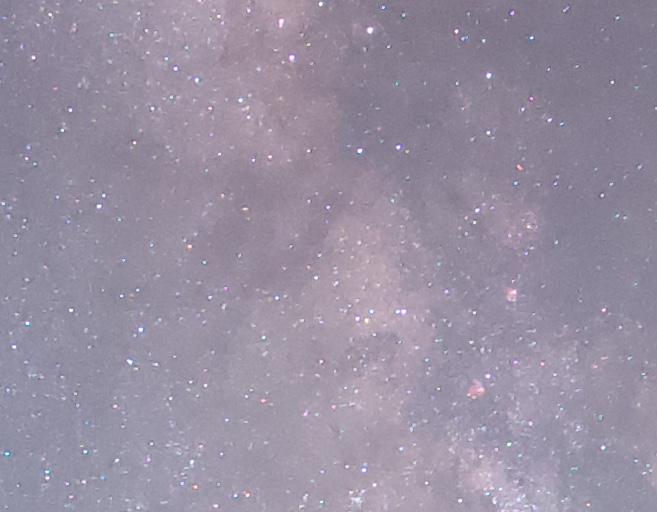
\includegraphics[width=\linewidth]{figures/photo_single_crop}\\[0.3ex]
  {\small 1枚だけの写真（一部を拡大）}
\end{minipage}\hfill
\begin{minipage}[t]{0.485\linewidth}\centering
  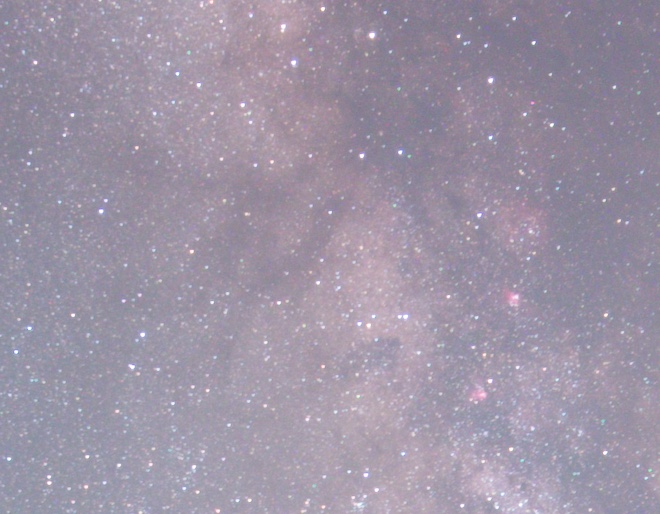
\includegraphics[width=\linewidth]{figures/photo_stacked_crop}\\[0.3ex]
  {\small 25枚をスタッキングした結果（同じ所）}
\end{minipage}
\caption{スタッキングするとノイズが減り、星と天の川がなめらかになります}
\end{figure}

\subsection{はじめに知っておきたい言葉}

このガイドでは、次の言葉を使います。

\begin{center}
\small
\begin{tabularx}{\linewidth}{>{\bfseries}l X}
\toprule
言葉 & 意味 \\
\midrule
スタッキング（合成） & 何枚もの写真を重ね合わせて1枚にすること。 \\
Light（ライト） & 星空を撮った、合成したい写真そのもの。 \\
Dark（ダーク） & レンズにキャップをして、Light と同じ設定（露出時間・ISO・温度）で撮った真っ暗な写真。センサーのむらや熱によるノイズを差し引くのに使います（なくてもかまいません）。 \\
Flat（フラット） & 明るさが均一な面（白い布や夜明け前の空など）を撮った写真。周辺が暗くなる「周辺減光」やごみの影を補正します（なくてもかまいません）。 \\
Bias（バイアス） & キャップをして、いちばん短い露出時間で撮った写真。センサーの基準の明るさを差し引きます（なくてもかまいません）。 \\
基準画像 & 位置を合わせるときの「お手本」にする1枚。ファイルリストの\ui{★}で選びます。 \\
アライメント & 写真ごとの星の位置のずれを合わせること（位置合わせ）。 \\
RAW / DNG & カメラが記録する、現像前のデータ（CR2・NEF・ARW など）。DNG は Adobe が決めた RAW の形式です。 \\
新星景 & 星空と地上の風景を1枚に収めた写真。星に合わせると地上が、地上に合わせると星がぶれるので、空と地上を分けて合成します。 \\
比較明合成 & 写真を重ねるとき、画素ごとにいちばん明るい値を残す合成。星の軌跡（スタートレイル）になります。 \\
\bottomrule
\end{tabularx}
\end{center}

\subsection{動作環境}\label{sec:requirements}

MacStarStacker には、動かす Mac に合わせた2つの版があります。どちらも同じ機能が使えます。

\begin{center}
\small
\begin{tabularx}{\linewidth}{l X}
\toprule
版（DMG の名前） & 動く Mac \\
\midrule
\textsf{macOS14-Universal} & macOS 14 (Sonoma) 以降の Mac（Apple シリコン・Intel のどちらも） \\
\textsf{macOS10.13-Universal} & Intel の Mac は macOS 10.13 (High Sierra) 以降、Apple シリコンの Mac は macOS 11 以降 \\
\bottomrule
\end{tabularx}
\end{center}

\begin{memo}[どちらを選べばいい？]
macOS 14 以降の Mac では \textsf{macOS14} 版を使ってください。それより古い macOS の Mac では \textsf{macOS10.13} 版を使います。
\end{memo}

読み込める写真は次のとおりです。
\begin{itemize}[itemsep=0.2ex]
  \item RAW：Canon（CR2・CR3）、Nikon（NEF）、Sony（ARW）、Fujifilm（RAF）、OM System / Olympus（ORF）、Panasonic（RW2）、Pentax（PEF）、DNG
  \item そのほか：TIFF、FITS、JPEG、PNG、HEIC
\end{itemize}

\begin{hint}[メモリの目安]
中央値合成やシグマクリッピング、新星景モードは、全部の写真のデータを一度にメモリに置くため、たくさんのメモリを使います。
2000万画素の RAW を20〜30枚なら、16GB 以上のメモリがあると安心です。足りないときは、始める前にメッセージでお知らせします。
\end{hint}
